	
	\documentclass[12pt,journal,compsoc]{IEEEtran}
	\usepackage[utf8]{inputenc}

	% *** CITATION PACKAGES ***
	\usepackage[nocompress]{cite}
	%\usepackage{cite}

	% *** GRAPHICS RELATED PACKAGES ***
	\usepackage[pdftex]{graphicx}
	\usepackage{framed}
	\graphicspath{{img/}}
	\DeclareGraphicsExtensions{.pdf,.jpeg,.jpg,.png}

	% *** MATH PACKAGES ***
	\usepackage[cmex10]{amsmath}

	% *** SPECIALIZED LIST PACKAGES ***
	\usepackage[footnote]{acronym}
	\usepackage{algorithm2e}
	\usepackage{alltt}

	% *** ALIGNMENT PACKAGES ***
	\usepackage{array}
	\usepackage{mdwmath}
	\usepackage{mdwtab}
	\usepackage{eqparbox}

	% *** SUBFIGURE PACKAGES ***
	\usepackage[caption=false,font=normalsize,labelfont=sf,textfont=sf]{subfig}
	%\usepackage[caption=false,font=footnotesize]{subfig}

	% *** FLOAT PACKAGES ***
	\usepackage{dblfloatfix}

	% *** PDF, URL AND HYPERLINK PACKAGES ***
	\usepackage{url}

	\newcommand\MYhyperrefoptions{bookmarks=true,bookmarksnumbered=true,
	pdfpagemode={UseOutlines},plainpages=false,pdfpagelabels=true,
	colorlinks=true,linkcolor={black},citecolor={black},urlcolor={black},
	pdftitle={Efficient 3D Isotropic Volume Reconstruction Based On 2D Localized Ultrasound Images},
	pdfsubject={Introduction To Lab Research},
	pdfauthor={Keck Jean-Baptiste},
	pdfkeywords={Introduction to Lab Research, Arthrosis, GPGPU, Ultrasound Imaging, Isotropic Volume Reconstruction}}

        \acrodef{gpgpu}[GPGPU]{General Purpose Computing on Graphics Processing Unit}
        \acrodef{cuda}[CUDA]{Compute Unified Device Architecture}
        \acrodef{timcimag}[TIMC-IMAG]{Techniques de l’Ingénierie Médicale et de la Complexité - Informatique, Mathématiques et Applications, Grenoble}
        \acrodef{gmcao}[GMCAO]{Gestes Médico-Chirurgicaux Assistés par Ordinateur}
	\acrodef{ssd}[SSD]{Solid-State Drive}
	\acrodef{hdd}[HDD]{Hard Disk Drive}
	\acrodef{simd}[SIMD]{Single Instruction, Multiple Data}

	\begin{document}

	\title{Efficient 3D Isotropic Volume Reconstruction Based On 2D Localized Ultrasound Images}
	

	\author{Jean-Baptiste Keck,~\IEEEmembership{Student,~Ensimag}\\
		Matthieu Chabanas,~\IEEEmembership{Supervisor,~TIMC-IMAG Laboratory}


	\IEEEcompsocitemizethanks{
	\IEEEcompsocthanksitem M. ~Keck is a student at Ensimag, Grenoble, France.
	\IEEEcompsocthanksitem M. ~Chabanas is in the team Gestes Médico-Chirurgicaux Assistés par Ordinateur in the TIMC-IMAG Laboratory, University of Grenoble, France.}
	
	\IEEEspecialpapernotice{TIMC-IMAG}
	\IEEEtitleabstractindextext{%
	\begin{abstract}
		A miniature 3D tracked ultrasonic probe has been developped to aquire intra-articular cartilage images under artroscopic chirurgy conditions. The aim is to detect cartilaginous lesions (arthrosis) and quantize their precise sizes and locations to help the clinician in his diagnostic and his therapeutic decision making.
		The ultrasonic transducer is tracked by an optical sensor, wich permits to find location and orientation of each 2D US images in a common 3D spacial reference. Near two thousands images are acquired when scanning a cartilage surface. An interesting tool is to rebuild a 3D isotropic volume (cubic voxels) with those images, allowing further processing.
		Conventional 3D ultrasound algorithms have low computational complexity but the huge amount of data generated makes it difficult to compute results within reasonable time on classical computers. In this paper we investigate the possibilities of regenerating a 3D isotropic volume with the help of \ac{gpgpu} (\ac{cuda}) by adaptating existing algorithms to massive parallelism provided by modern everyday GPUs.
	\end{abstract}

	\begin{IEEEkeywords}
		Introduction to Lab Research, Arthrosis, \acl{gpgpu}, Ultrasound Imaging, Isotropic Volume Reconstruction.
	\end{IEEEkeywords}
	}}	
	
\maketitle
\markboth{Introduction to Laboratory Research, Report,~Version.~1, No.~1, May~2014}

% make the title area

\section{Introduction}

\IEEEPARstart{F}{reehand} three-dimentional ultrasound imaging is a highly attractive research area because it is capable of volumetric visualization and analysis of tissue and organs. Conventional two-dimentional ultrasound imaging has been widely used for many clinical applications such as medical diagnosis and image-guided surgery. In comparisson with Computed Tomography (CT) and Magnetic Resonance Imaging (MRI), ultrasound imaging is non invasive, real time, portable and low cost. However, 2D ultrasound imaging fails to offer clinicians whole volume data for visualization and analysis. Thus three-dimensional ultrasound imaging systems has been developped to overcome those limitations by constructing various 3D datasets. Several approaches for constructing 3D ultrasound volume data have been reported. These approaches can be classified into three categories : dedicated 3D probes, mechanical scanning approach, and freehand scaning approach. 
Dedicated 3D probes can provide 3D data in real time but they are expensive and have limitations in scanning large volume organs.
The mechanical scanning approaches usually use conventionals 2D transducers wich are translated and rotated with stepping motors. This design creates limitations in term of their scanning range. 
Finally, freehand ultrasound use conventionals 2D tranducers in pair with a positioning sensor to save position and orientation of each acquired image.
Freehand 3D ultrasound has received increasing attention for it's low-cost and flexibility, as it allows the user to manipulate and view the desired anatomical section freely.
During scanning a sequence of US images are captured along with their positions and orientations, asynchronously. Those datas are then used to reconstruct a 3D volume by using various interpolation or approximation algorithms. The reconstruction algorithm plays a key role in the construction of three-dimentional ultrasound volume data with higher image quality and faster reconstruction speed.\\

TODO\\

Even if conventional 3D reconstruction algorithms have low computational complexity, the huge amount of data generated by a single scan (thousands of 2D images) makes it difficult to compute volume data in reasonable clinical time on classical computers.
This paper aims to speed up 3D volume processing by adapting existing reconstruction algorithms to the massive parallelism provided by nowadays affordable GPUs. This is achieved throught \acl{gpgpu} (\ac{gpgpu}), a concept that has been well developped and widely adopted during the last decade and that continues its growth.
The Open Computing Language (OpenCL) is the currently dominant open general-purpose GPU computing language. The dominant proprietary framework is the \acl{cuda} (\ac{cuda}).
Althought \ac{cuda} requires a Nvidia CUDA compatible graphic card, we choose it because of its more mature status (performance and debugging tools) but algorithms are easily adaptable to OpenCL as well, allowing executions on Nvidia's and AMD's graphic cards, and even Integrated Graphics Processors (IGPs).

\section{System overview}

\subsection{System setup}

The freehand 3D ultrasound imaging system consits of three modules : a 2D ultrasound scanner specially designed to acquire intra-articular cartilage US images under artroscopic chirurgy conditions, an optical position and orientation sensor and a work station with custom-designed software for data-aquisition. The volume reconstruction is for the moment done as a post-process in another specially-designed piece of software.
The portable ultrasound scanner concists of 64 axis-aligned transducers. Althought it is a freehand system, the axe is slightly rotated by a stepper motor to achieve a greater scanning area. The transformation due to the rotation of the motor is taken in account.

\begin{figure}[!h]
\centering
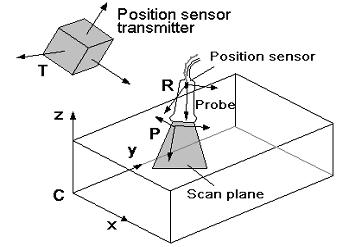
\includegraphics[width=2.5in]{freehand}
\caption{A classical freehand ultrasound imaging system setup}
\label{fig_1}
\end{figure}

The receiver of the spacial sensing device is attached to the hand-help probe of the ultrasound scanner.
During data acquisition, spacial data and digitalized 2D scans are simulteanously recorded and collected.
Since the ultrasound probe and the spacial sensor are independent, the temporal delay between two data streams can not be avoided.

\subsection{Data acquisition}

After signal processing 2D slices of logical size $L_x$ x $L_y = 64$x$1296$ pixels are generated. 
As the transducers are $\epsilon_x=205\mu m$ wide, the images have a physical size of $P_x = 64\;\epsilon_x=19.12mm$. 
The precision on the other axe is $\epsilon_y=18\mu m$, and thus the images have a physical height of $P_y = 1296\;\epsilon_y=23.328mm$.
For the images we will use this convention : we place the origin at the top-left with the x-axis oriented towards the right and the y-axis oriented towards the bottom. 
We define $X_p=(x_p,y_p,0,1)^T$ the homogenous vector that describes logical position of each pixel $(x_p,y_p)$ in an image whose origin is at $(O_x,O_y)$. 
$S_x$ and $S_y$ are the pixel spacing on each axis and are defined as $S_x = \frac{P_x}{L_x}$ and $S_y = \frac{P_y}{L_y}$. 

\begin{equation}
	M_{model} = \left(
	\begin{IEEEeqnarraybox*}[][c]{,c/c/c/c,}
		$$
		S_x&0&0&O_x\\
		0&S_y&0&O_y\\
		0&0&0&0\\
		0&0&0&1%
		$$
	\end{IEEEeqnarraybox*}
\right)
\end{equation}

The physical position of each pixel in its local physical coordinate system can be calculated as the following : 
\begin{IEEEeqnarray}{rCl}
X_m = M_{model}\;X_p 
\end{IEEEeqnarray}

\begin{figure}[!h]
\centering
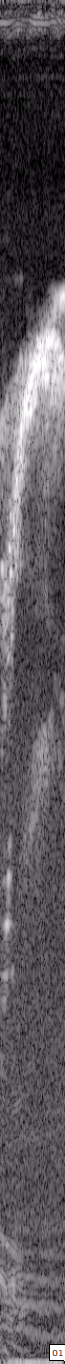
\includegraphics[width=40mm, height=50mm]{scan}
\caption{A typical 2D ultrasound image of intra articular cartilage. The white band is the cartilage itself.}
\label{fig_2}
\end{figure}

$M_{RP}$ is the transformation matrix from the optical position sensor reflector (R) to origin of the scanned image plane (P), $M_{ER}$ is the transformation matrix from the optical emitter (E) to (R) and $M_{VE}$ is the transformation matrix from the voxel coordinate of the reconstructed volume (V) to (E). Note that all those matrices are 4x4 homogeneous matrices.

$M_{RP}$ is initially unknown and must be obtained through a calibration process TODO.

With those matrices and (1), the whole forward transformation can be written as : 

\begin{IEEEeqnarray}{rCl}
	X_v = M_{VE}M_{ER}M_{RP}\;X_m = M\;M_{model}\;X_p
\end{IEEEeqnarray}

The specially designed sofware used to acquire data can export each image data in a raw file which includes single precision float image data, and a mhd file which include a path to the corresponding raw file and the transformation matrix M.

\section{Volume Reconstruction}

\subsection{Reconstruction steps}

After the 2D images and positions are exported as raw and mhd files, the next procedure is to reconstruct a 3D volume data. 
The sampled images are denoted \{$I_i$\} and the transformations matrices \{$M_i$\}.

\newpage
Here is the flow diagram of freehand 3D ultrasound volume reconstruction :
\begin{framed}
\noindent\textbf{Step 1 : Data loading}
\begin{itemize}
	\item Parse mhd files
	\item Load raw images
	\item Load transformations
\end{itemize}
\textbf{Step 2 : Data preprocessing}
\begin{itemize}
	\item Position filtering
	\item Image filtering
	\item Image cropping
	\item Image data conversion
\end{itemize}
\textbf{Step 3 : Grid construction}
\begin{itemize}
	\item Determinate grid size
\end{itemize}
\textbf{Step 4 : Volume Filling}
\begin{itemize}
	\item Bin-filling
	\item Hole-filling
\end{itemize}
\end{framed}

\subsection{Data loading}

Loading data is not as easy as one might think and can rapidly become a serious bottleneck compared to what GPGPU can provide in terms of speedup. 
As each US scan is exported in its own mhd and raw file, thousands of mhd files have to be parsed to get each transformation matrix \{$M_i$\} and get the path to the corresponding image data and load the raw image \{$I_i$\}.  
With two thousands images this operation can easily take 2 minutes on regular \ac{hdd} and even half a minute on a \ac{ssd}.
One easy fix would be to merge all the image data into a single raw file, and the transformation matrices in another raw file as well, or simply keep the generated data in the computer memory when doing on the fly or immediate postprocessing.
Data locality is something we do not only want on the disk, but in the memory too. This introduces an important concept : Array of Structures (AoS) versus Structure of Arrays (SoA). In GPGPU, memory accesses are a serious bottleneck when done improperly and SoA are often the better solution than AoS. 

For example, a list of 3D vectors can be represented with 3 arrays, one for each of its coordinates (SoA), or with an array of 3D vector structures (AoS) :

\begin{samepage}
\begin{alltt}
\textbf{Structure of Arrays (SoA):}
struct vectors \{
    float x[100];
    float y[100];
    float z[100];
\}

struct vectors v;

\textbf{Array of Structures (AoS):}
struct vector \{
    float x;
    float y;
    float z;
\}

struct vector v[100]
\end{alltt}
\end{samepage}

When using a structure of arrays we have memory spacial locality between each of the vector coordinates. When a memory read occur in the global memory of a GPU, a large chunk of data is read (most of the time 256 bytes memory segments aligned on 256-byte adress). This is because the GPU is a massive parralel architecture.
In \ac{cuda}, threads are grouped into thread blocks, which are assigned to multiprocessors on the device. During execution there is a finer grouping of threads into warps. Multiprocessors on the GPU execute instructions for each warp in \acl{simd} fashion. The warp size of current CUDA-capable GPUs is 32 threads. 
The device coalesces global memory loads and stores issued by threads of a warp into as few transactions as possible to minimize memory bandwidth.
Any misaligned access by a half warp of threads results in 16 separate 32-byte transactions. If only 4 bytes are requested per 32-byte transaction (a simple integer or float), we should expect the effective bandwidth to be reduced by a factor of eight.
For strided global memory access things get even worse, and get worser when the stride get bigger.
That is not surprising because when concurrent threads simultaneously access memory addresses that are very far apart in physical memory, then there is no chance for the hardware to combine the accesses.
Strides entailed by Array of Structures is the reason why we want to use Structure of Arrays, where data is nicely arranged to be accessed in a parallel manner.

Taking this into account, we decompose the 4x4 homogeneous transformation matrices \{$M_i$\} into a structure of 12 arrays, the 3x3 inner transformation matrix coefficients $r^1$ through $r^9$, and the 3D offset vector coefficients $(x,y,z)$ :

\begin{equation}
	M_i = \left(
	\begin{IEEEeqnarraybox*}[][c]{,c/c/c/c,}
		$$
		r_i^1&r_i^2&r_i^3&x_i\\
		r_i^4&r_i^3&r_i^5&y_i\\
		r_i^5&r_i^6&r_i^7&z_i\\
		0&0&0&1%
		$$
	\end{IEEEeqnarraybox*}
\right)
\end{equation}

The matrix is initially stored in a row-major manner, this is why we use such indexing convention for $r_i$.

\begin{samepage}
\begin{alltt}
\textbf{The resulting struct is :}
struct transformations \{
    //offsets
    float *x;
    float *y;
    float *z;

    //3x3 matrix coefficients
    float *r1;
    float *r2;
    ...
    float *r9;
\}

\end{alltt}
\end{samepage}

Image data do not recquire such memory reorganization as it is already stored and loaded as a row-major matrix of black and white pixels represented by simple precision floats. We just pay a special care to load the images in a big contiguous memory space and not to load them at random locations into the memory.
Of course if the images were color images, we would have separated the red, green and blue channels into three separate arrays in a SoA manner. \par

This is not the only thing to take into account when loading data into memory when using GPGPU.
When allocating CPU memory (RAM) that will be used to transfer data to the GPU memory (VRAM) for computing purpose, there are two types of memory to choose from : pinned and non-pinned memory. 
Pinned memory is memory specially allocated with a GPGPU dedicated malloc function (cudaMallocHost in CUDA), which prevents the memory from being swapped out and provides improved transfer speeds. 
Non-pinned memory is memory allocated using the classical malloc function in C, or using the new operator in C++. 
Pinned memory is much more expensive to allocate and deallocate but provides higher transfer throughput for large memory transfers.
Empirically, using pinned memory only makes sense when the amount of memory transferred each way is larger than 16 MB (TODO). 
In our case with 2000 US scans, we have 664MB of float images, and 96Ko of transformations data so we just go for the pinned memory for the images. \par

At the end of this step, we have 12 arrays of transformation coefficients stored contiguously in the CPU memory in a non pinned manner, and one big contiguous array of floats representing the images that is pinned in the CPU memory. 

\subsection{Data preprocessing}


Data preprocessing include image cropping, position filtering and image filtering.\par

Sometimes it is needed to crop the ultrasound images to select a region of interest. When doing this, we must not forget to keep or update image offset in local image coordinates for further processing. 

Position filtering is needed because the position sensor device is susceptible to interferences and because our minitature probe was prone to bending. Thus the variation of probe position between consecutive slices can not be avoided. TODO\par

Volume reconstruction algorithms recquire accurate edge maps for good performance, howewer highly signal dependant nature of ultrasound speckle makes these difficult to obtain. Various filtering techniques have been developped to suppress speckles in order to improve the quality of images. 
Among them, the nonlinear filters have recently received an increasing interest, due to some of their important capabilities over linear filters. For example, A. Babakhani \textit{et al.}\cite{1} proposed in 2006 an extensive comparisson of such non linear filters applied to ultrasound imaging and 3D volume reconstruction, including non linear gaussian diffusion filters (NLG), anisotropic filters with level set (ANL), offset filters with level set (OFS) and pure morphological filters (PUM).\par

Due to a lack of time on this project, neither signal filtering nor image filtering have been considered here even if such filtering is possible on modern GPUs.

Most of current and past years GPUs have 512MB to 2GB embedded memory (VRAM). Thus a high volume of image data can be problematic when doing volume reconstruction on GPU because the grid needed to reconstruct the volume has to be stored too and memory should be kept for the GPU program execution stack. In addition to that, memory is already taken by the system through the graphic card driver when using a graphical desktop environment. 
One simple solution is to execute the algorithm on the GPU with smaller group of images each after another but transferring data from CPU memory to GPU memory is rather time-consuming. 
Typical transfer rates are 3Gbps for non-pinned memory and 6Gbps for pinned memory.
We chose an even simpler method for reducing images impact on memory : For now our image were represented as an array of floats between 0.0 and 255.0 but we don't need such precision. Thus we decided to convert our 4 bytes floats into 1 byte unsigned chars, letting the initial 664MB images memory footprint fall down to only 166MB. This is done in a simple CUDA kernel, as it is a trivially parallelizable operation. To do this, we just have to allocate two arrays, a 166MB pinned memory array on the CPU and a 166MB memory array on the GPU, transfer initial float data to GPU memory, execute the kernel, transfer back the casted data to the CPU memory and finally free the old float datas on CPU and GPU. 

\begin{figure}[!h]
\centering
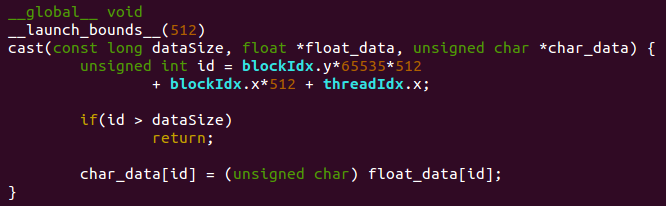
\includegraphics[width=3.5in]{simple_kernel}
\caption{A simple CUDA kernel example performing image data conversion from float to unsigned char.}
\label{kernel}
\end{figure}

Fig.\ref{kernel} shows a simple kernel performing this operation. Note the \ac{simd} coding style : there are simultaneous parallel computations, but only a single instruction at a given moment. Lets say $N_i$ is the number of images we loaded at the first step. 
The $dataSize$ variable counts the total number of pixels ($dataSize=N_i$x$L_x$x$L_y$ assuming we did not crop anything) and the $id$ is a variable designating the current thread, starting at 0. Since the max $id$ can exceed the number of pixels $dataSize$, a simple if statement prevent the program to access prohibited memory. 

\subsection{Grid construction}

\subsubsection{Computing bounding box}
The third step in the reconstruction procedure is the establishment of coordinate system configuration for the reconstruction including its origin, its dimension and volume grid spacing. As our system has no need to predefine a volume before data acquisition we can use a simple bounding box technique as proposed by T. Wen \textit{et al.} \cite{2}.

A bounding box can be represented with two points only, $X_{min} = (x_{min},y_{min},z_{min})^T$ and $X_{max} = (x_{max}, y_{max}, z_{max})^T$.

With the notations of Eq.2 and Eq.3, the algorithm to find the bounding box is pretty simple :

\begin{algorithm}
	\KwData{$X_{min} = (+\infty,+\infty, +\infty)$
		$X_{max} = (-\infty,-\infty, -\infty)$}
	\For{each image $I_i$}{
		\For{each of the four corner vertice $v_j$ of $I_i$}{
			$X_p^j$ = image coordinate of $v_j$;
			$X_v^j = M_i\;M_{model}\;X_p^j$\;
			\If{point $X_v^j$ outside of the bounding box}{Update $X_{min}$ and $X_{max}$\;}
		}
	}
\end{algorithm}
	
The test to know wether the point is in the bounding box or not concists of 6 scalar comparisons, and thus this algorithm can be executed safely on CPU without any performance drawbacks.
The origin of the volume is then placed at $X_{min}$.

At the end of this algorithm, all US images are contained in this bounding box and $X_{min}$ and $X_{max}$ are atteigned by one ultrasound image corner at least once.


\begin{figure}[h!]
\centering
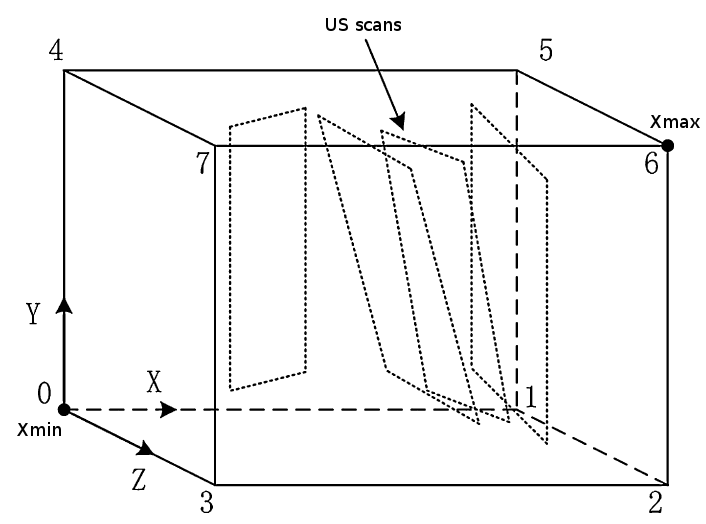
\includegraphics[width=3.5in]{bounding_box}
\caption{The resulting bounding box defined by $X_{min}$ and $X_{max}$.}
\label{fig_2}
\end{figure}

The next step is to choose a voxel size. This is a critical parameter because the memory footprint of the grid is what hinders GPGPU volume reconstruction. 

\subsubsection{Choosing a voxel size}

Lets assume $W_b$x$H_b$x$L_b$ are the width, height and length of the generated bounding box, $W_g$x$H_g$x$L_g$ are the width, height and length of the grid (in voxels) and $\delta_v$ is the cubic voxel size. With those notations, we need to allocate at least a grid of $N_v = W_g$x$H_g$x$L_g =  \dfrac{W_b}{\delta_v}$x$\dfrac{H_b}{\delta_v}$x$\dfrac{L_b}{\delta_v}$ voxels. \par

\vspace{0.2cm}
Thus, memory cost is cubical with the number of subdivisions $N_s$. Each time we want to double precision, we have to pay eight times more memory.

\begin{table}[!t]
\renewcommand{\arraystretch}{1.3}
%\extrarowheight 
\caption{Memory footprint for a $50$x$50$x$50$mm bounding box and unsigned char voxels}
\label{memory_table}
\centering
\begin{tabular}{|c|c||c|c||c|}
\hline
$log_2(N_s)$ & $N_s$ & $\delta_v (\mu m)$ & $N_v$ & Grid memory \\
\hline
12 & 4096 & 12.2 & $2^{36}$ & 68.7GB\\\hline
11 & 2048 & 24.4 & $2^{33}$ & 8.59GB\\\hline
10 & 1024 & 48.8 & $2^{30}$ & 1.07GB\\\hline
9 & 512 & 97 & $2^{27}$ & 134MB\\\hline
8 & 256 & 195 & $2^{24}$ & 16.8MB\\\hline
7 & 128 & 390 & $2^{21}$ & 2.1MB\\\hline
\end{tabular}
\end{table}
Table \ref{memory_table} shows grid memory consumption for a bounding box which is approximately the size of the bounding box obtained when scanning our intra-articular cartilage.
We see that when the voxel size $\delta_v$ goes under $0.1mm$ the memory begins to cause some problems to our GPU memory.
Even if some professional graphic cards can have up to 12GB of memory, a simple $\delta_v$ set to $0.05mm$ can cause trouble.
In fact, as it is explained later in this paper, even simple volume reconstruction algorithm will recquire at least four such grids in the bin-filling stage.

\begin{figure}[!h]
\centering
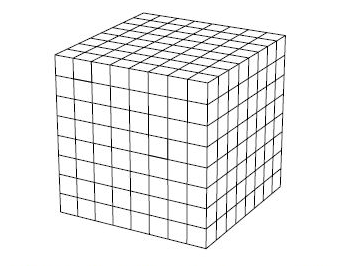
\includegraphics[width=2.5in]{grid}
\caption{A cubic bounding box split with $N_s=8$}
\label{fig_2}
\end{figure}

For example to perform an average in a \acl{simd} manner, we need at least two unsigned int grid and two unsigned char grids witch multiply the table \ref{memory_table} grid memory footprint by 10 when assuming unsigned int are 4 bytes and unsigned char 1 byte.
That means that $\delta_v=0.05mm$ entails at least $10.70GB$ memory consumption just for the grids on the GPU memory.
Adding to that the size of the images, the system graphical environment load and the execution stack and our 12GB professional graphic card wont survive under such memory load.

The only solution is to split the grid into subgrids on the GPU side, and keep the whole voxel grid on the CPU side. The amount of spliting depends of the graphic card free runtime memory and the reconstruction algorithm used.

\section{Volume Filling}
\subsection{Existing methods overview}
\subsection{Existing bin and hole-filling algorithms}

\section{Adapting volume filling to Cuda}


%\begin{figure*}[!t]
%\centering
%\subfloat[Case I]{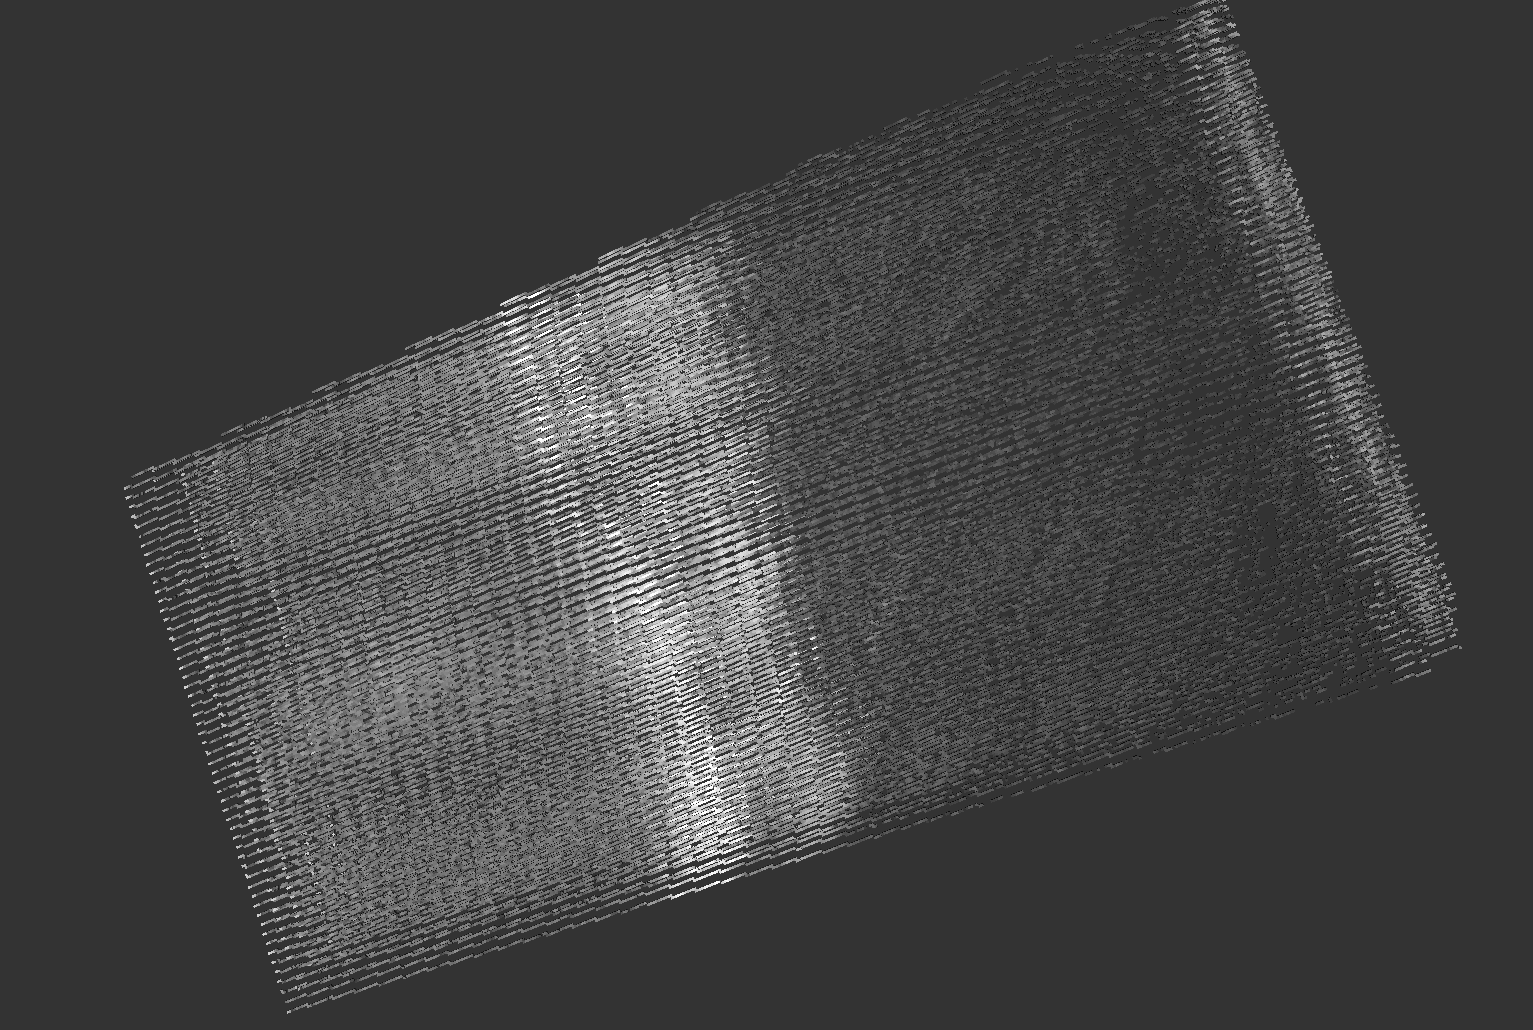
\includegraphics[width=1.5in]{data_0}%
%\label{fig_first_case}}
%\hfil
%\subfloat[Case II]{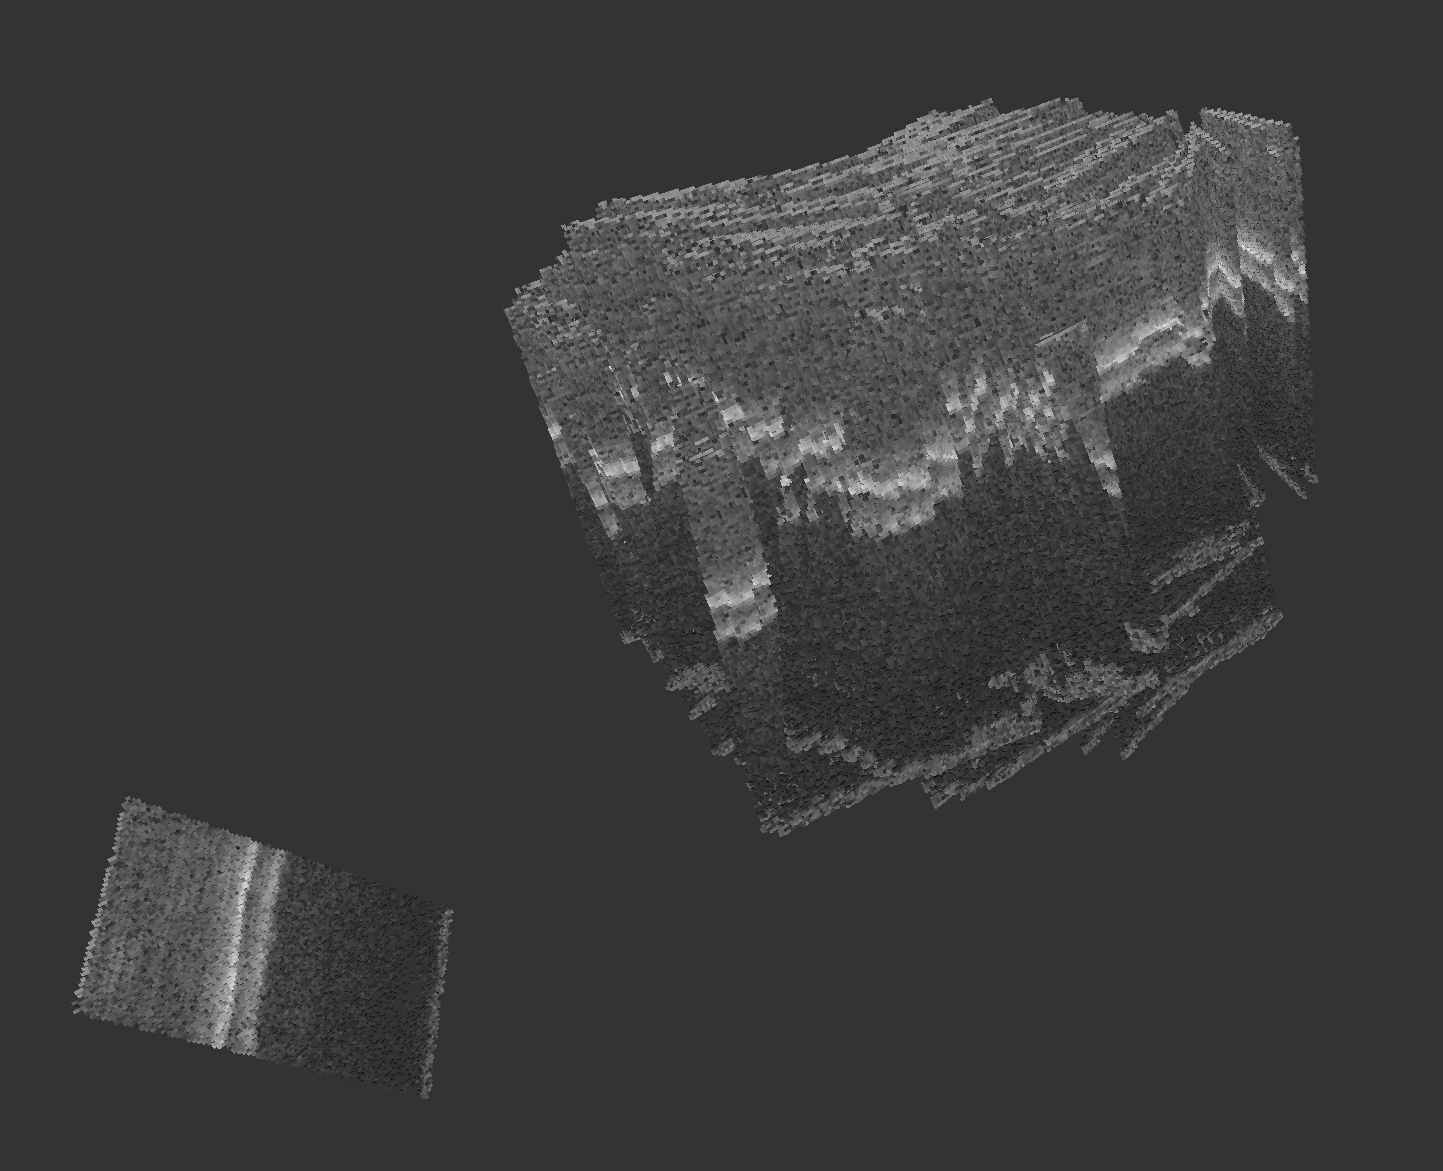
\includegraphics[width=1.5in]{data_1}%
%\label{fig_second_case}}
%\hfil
%\subfloat[Case III]{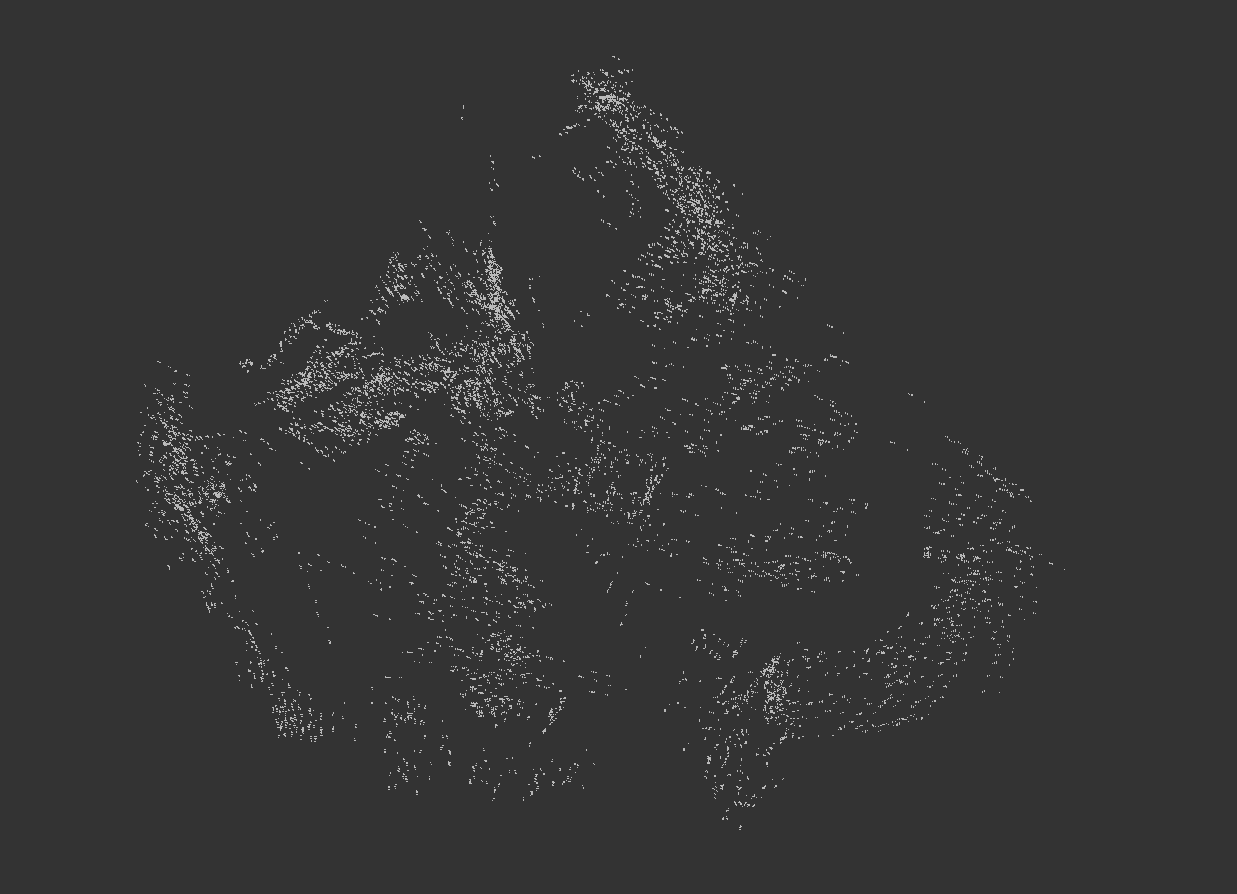
\includegraphics[width=1.5in]{femur_2}%
%\label{fig_third_case}}
%\caption{Simulation results.}
%\label{fig_sim2}
%\end{figure*}


\section{Conclusion}
The conclusion goes here.

\appendices
\section{Voxel Renderer}
Appendix text goes here.

\section*{Acknowledgments}
I would like to thank the TIMC-IMAG laboratory for having hosted me for 4 months, especially the GMCAO team members that were always here to help when there were any problems and for the good mood. Special thanks goes to M. Chabanas for having taken the time and energy throughout the project by providing precious feedbacks and for having introduced me to the TIMC-IMAG laboratory.

\cite{1}\cite{2}\cite{3}\cite{4}\cite{5}\cite{6}\cite{7}.

\bibliographystyle{IEEEtran}
\bibliography{master}

%\begin{IEEEbiography}[{\includegraphics[width=1in,height=1.25in,clip,keepaspectratio]{mshell}}]{Michael Shell}
%\begin{IEEEbiography}{Michael Shell}
%Biography text here.
%\end{IEEEbiography}

%\begin{IEEEbiographynophoto}{Jane Doe}
%Biography text here.
%\end{IEEEbiographynophoto}
%\vfill

\end{document}
